\documentclass[a4paper,12pt]{article}
\usepackage{../../../mypackages}
\usepackage{../../../macros}

\setlength{\parindent}{0pt}


\begin{document}

\title{Chapitre 4 : L'atome - Projet de fin de chapitre}
\author{N. Bancel}
\date{Septembre 2024}
\maketitle

\section*{L'humanité dans un dé à coudre}


%colback=green!10!white, colframe=green!75!black


\begin{tcolorbox}[colback=gray!30, colframe=black]
  \textbf{Notes} : Cet exercice est volontairement peu guidé, il nécessite de formuler un problème de manière indépendante. Pour autant : ne pas hésiter à solliciter un/une camarade de classe, ou me solliciter directement. \par
  \vspace{1em}
  Notions abordées / Compétences à mettre en place :
  \begin{itemize}[noitemsep]
    \item Dimensions atomiques
    \item Poser un problème / Définir les variables qui permettent sa résolution
    \item Faire des estimations / Formuler des hypothèses
    \item Interpréter des résultats
    \item Challenger un modèle 
  \end{itemize}
  \end{tcolorbox}

\subsection*{Enoncé}

Frédéric Joliot, époux d'Irène Curie, fille de Pierre et Marie Curie, physicien et chimiste, également Prix Nobel, utilisait cette image : \par 
\vspace{1em}
\textit{"Si on pressait les uns contre les autres les noyaux des atomes de toute l'humanité, ils occuperaient un volume inférieur à celui d'un dé à coudre"}. \par
\vspace{1em}
Cette affirmation est-elle correcte ?

\subsection*{Hypothèses - Informations}

\begin{itemize}[noitemsep]
  \item Dans la citation ci-dessus, l'"humanité" fait référence à l'ensemble des êtres humains sur la terre
  \item On considèrera que la masse moyenne d'un individu est de 50 kg 
  \item On considèrera que l'être humain est composé des atomes suivants, dans les proportions indiquées dans le tableau ci-dessous : \par
  \vspace{1em}
  \begin{tabular}{lcccc}
    \toprule
    & \textbf{C} & \textbf{O} & \textbf{H} & \textbf{N} \\
    \midrule
    \textbf{Abondance massique} & 20\% & 67\% & 10\% & 3\% \\
    \textbf{Masse des atomes (en kg)} & \( 20 \times 10^{-27} \) & \( 27 \times 10^{-27} \) & \( 1.7 \times 10^{-27} \) & \( 23 \times 10^{-27} \) \\
    \bottomrule
\end{tabular}
\vspace{1em}

  \item Dans ce "dé à coudre", on considère que les noyaux des atomes peuvent se compresser les uns contre les autres dans la configuration suivante : 
  
  \begin{figure}[H]
    \centering
    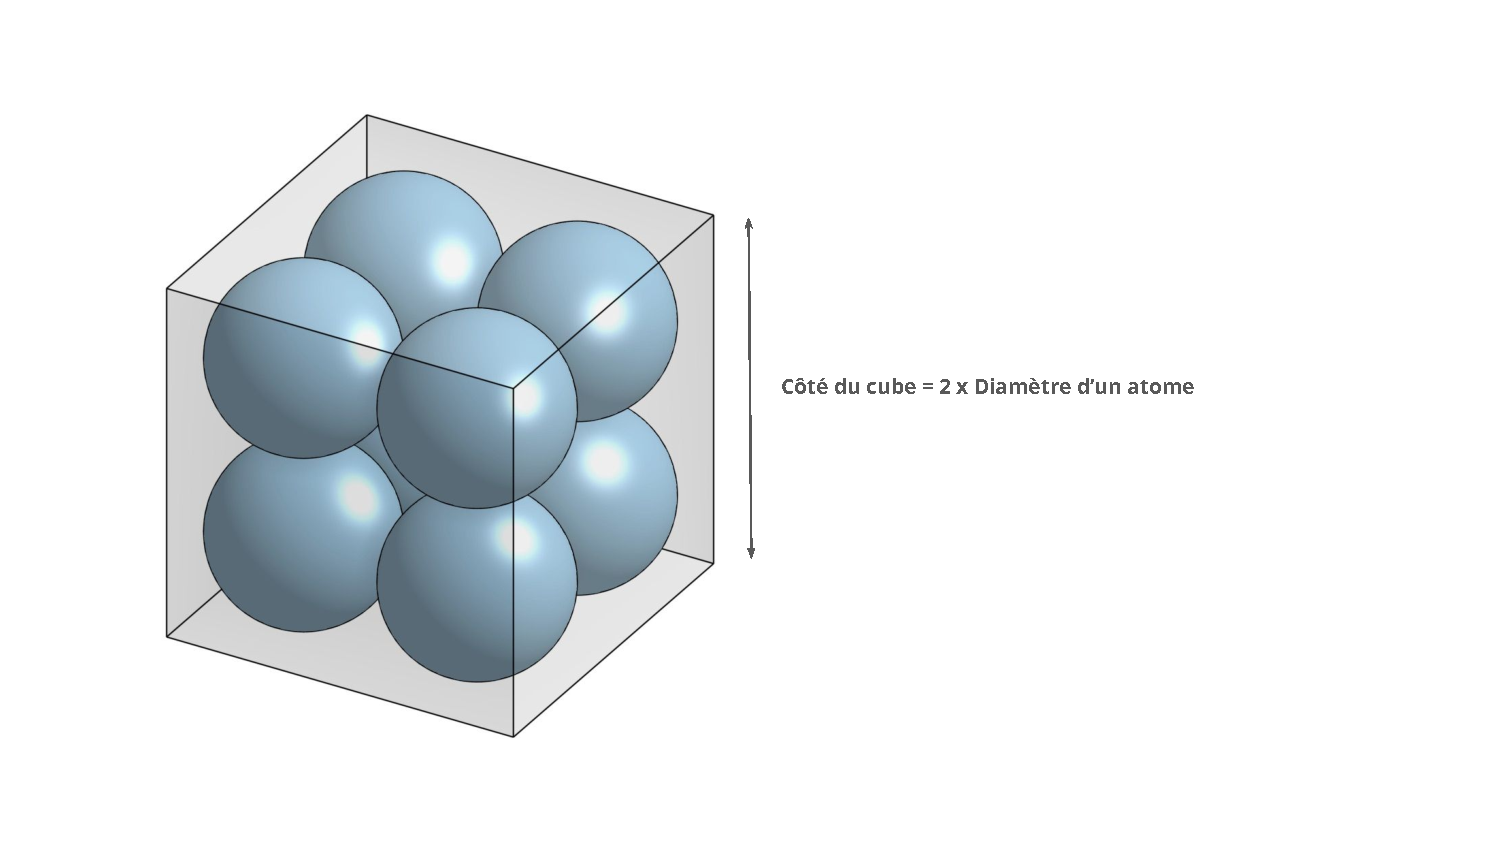
\includegraphics[width=0.8\linewidth]{Projet Atome.pdf}
    \caption{\label{} Disposition des noyaux des atomes}
  \end{figure}

\end{itemize}

\subsection*{Interprétation / Questions supplémentaires}

\begin{itemize}[noitemsep]
  \item Que peut-on en déduire quant au fait qu'on dit souvent que la matière est essentiellement composée de vide ?
  \item On appelle \textbf{compacité (ou taux de remplissage)} d'un regroupement d'atomes la fraction que les sphères de leurs noyaux occupent au sein d'un volume donné. Le volume étant ici le cube gris clair, quelle proportion de ce cube est occupée par de la matière (les noyaux) ? Cette compacité se note 
  
\begin{figure}[H]
  \centering
  \[ c = \frac{V_s}{V} \]
  \begin{tabular}{@{}>{$}l<{$}l@{}}
    c & compacité ("taux réel d'occupation de l'espace")\\
    V_s & Volume occupé par les noyaux au sein du cube \\
    V & Volume du cube qui englobe les noyaux \\
  \end{tabular}
\end{figure}

\item Question bonus : en cherchant sur Internet de l'information sur les structures cristallines, quelle agencement d'atomes dans l'espace permet de maximiser cette compacité ? Quelle est la valeur de cette compacité ? La comparer avec la compacité du modèle que nous avons choisi dans ce projet.

\end{itemize}




\end{document}
